\documentclass{article}

\usepackage[margin=1in, includefoot]{geometry} % Margins Setup
\usepackage[hidelinks]{hyperref} % Allows for Clickable References
\usepackage{multicol}
\usepackage{amsmath}

% Graphics Dependencies
\usepackage[]{graphicx} % Allows Image Imports
\usepackage[]{float} % Allows Control of Float Positions
% Table Dependencies
\usepackage{tabulary} % helps with table width formatting and text wrapping in tables
\usepackage[none]{hyphenat} % keeps words from breaking up in tables
% Bibliography Dependencies
\usepackage[numbers,sort&compress]{natbib} % Ensures Citation Numbers are in order (If Multiple)

% Lists Dependencies/Setup
\renewcommand{\labelitemi}{$\bullet$}
\renewcommand{\labelitemii}{$\diamond$}
\renewcommand{\labelitemiii}{$\circ$}

% Header/Footer Info
\usepackage[]{fancyhdr} % Header/Footer Setup
\pagestyle{fancy}
\fancyhead{}
\fancyfoot{}
\fancyfoot[R]{\thepage\ }
\renewcommand{\headrulewidth}{0px}
\renewcommand{\footrulewidth}{1px}

\begin{document}
    \begin{titlepage}
        \begin{center}
            \line(1,0){340} \\
            [5mm]
            \huge{\bfseries Correcting Binary Corruption in Matrix Multiplication Using C Programs} \\
            \line(1,0){340} \\
            [.25 in]
            \textsc{\LARGE Gupta College of Science} \\
            \textsc{\LARGE Coastal Carolina University} \\
            [.25 in]
            \textsc{\LARGE Colin Matz \\
            Junior B.S. Information Technology, \\ 
            Cybersecurity Minor \\
            December 2, 2022} \\
        \end{center}
    \end{titlepage}

    % Abstract Page
    \pagenumbering{roman}
    \section*{Abstract}\label{sec:abstract}
    \addcontentsline{toc}{section}{\numberline{}Abstract}
    While solving complex issues, computers have given us the ability to accomplish new advances that 
    we once never thought possible. However, due to the complexity of such programs, small errors in data
    can cause large discrepancies in outcomes. Since there are the possibilities of these small errors in
    programs, there must be code or programs that are tasked with solving this corruption. This paper will
    highlight and explain a possible solution via a program written in C that will simulate small data
    corruption and will react accordingly to fix such problems. This paper will also break down the methods
    needed in order to fix corruption errors within output files in order to be further used in future 
    computations.

    % \newpage

    % list of Figures/Tables
    \listoffigures
    \addcontentsline{toc}{section}{\numberline{}List of Figures}
    % \newpage

    \listoftables
    \addcontentsline{toc}{section}{\numberline{}List of Tables}
    \newpage

    % Table of Contents 
    \tableofcontents
    \thispagestyle{empty}

    % Main Body
    \newpage
    \pagenumbering{arabic}
    \setcounter{page}{1}

    % Actual Paper
    \begin{multicols}{2}
    \section{Introduction}\label{sec:intro}
    Super computers have been evolving rapidly in order to meet the ever-growing need for data computing
    in society. However, as society becomes more dependent on technology, arbitrary errors caused by means
    out of the control of the specialists watching over these supercomputers can have a much higher impact.
    This breeds the need for in depth error detection for even the smallest errors, such as an error known
    as "flipping" which is a change in a binary bit from a 0 to a 1 \cite{basgall}. Such an error, which at first glance seems like not a large issue, can have detrimental effects to a
    program being ran.

    % Test Figure / Example Figure
    \begin{figure}[H]
        \centering
        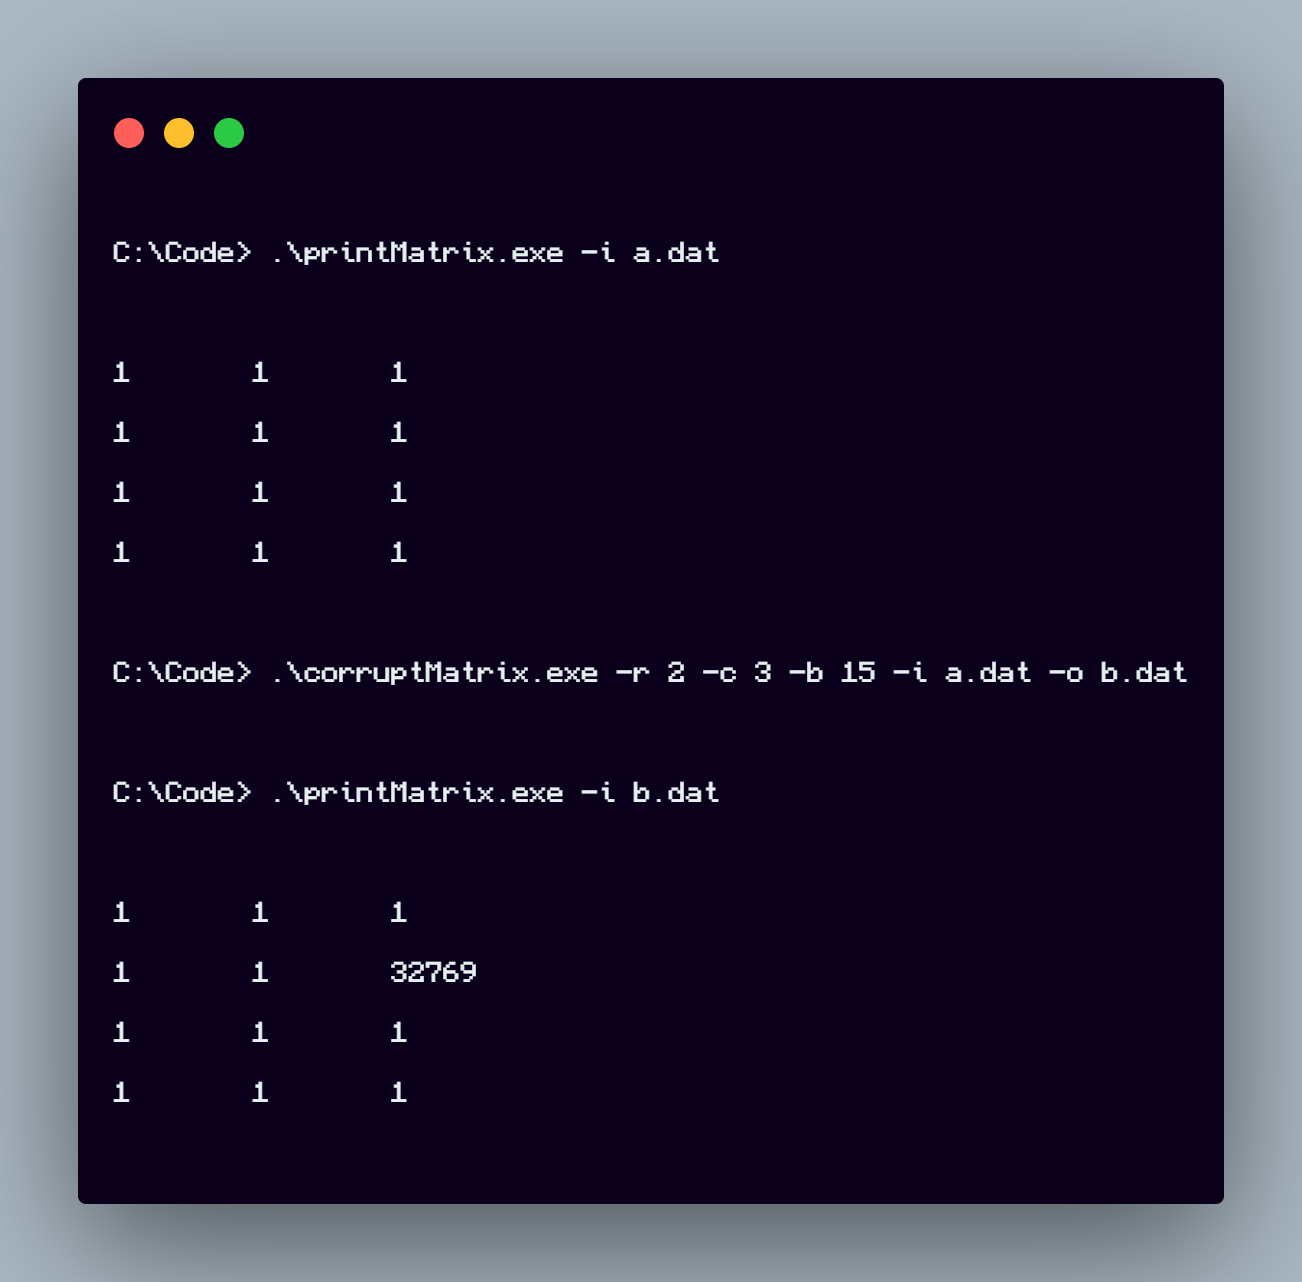
\includegraphics[height=2.75in]{./media/intro1.PNG}
        \caption[Corruption Example 1]{Corruption Example 1}
        \label{fig:CE1}
    \end{figure}

    Figure \ref{fig:CE1} shows a "flipping" event on the 15th bit of a number in a matrix.
    \vspace {4mm}
    
    
    looking at the above image, it is evident that the small bit change had a large impact and any attempt
    to use this data in further computations would lead to detrimental arithmetic errors. This can be combated
    as the program runs by doing a few checks of the data, but can cause problems when they are left unchecked.
    \section{Design}\label{sec:design}
    The program that has been built to emulate and solve this issue has multiple parts and functions to
    accomplish the data corruption and correction. Essentially, the program will start by creating two matrices
    and storing them into files. From there, the program will reopen each matrix individually and add a sum row 
    or column to use in future error checking. Then the two matrices will be multiplied. From there, the program
    will perform a bit flip on one of the numbers in the matrix resulting from the multiplication. Once this is
    done, the program will detect where the bit flip has occurred by comparing the values in the matrix with the
    sum row and column and will use that information to apply the correct value to the corrupted value. To accomplish
    this, the program will utilize several programs all sharing several functions. While this use case is not quite
    how it would be expected in current infrastructure, the methods should resemble the thinking technology specialists
    use in order to combat bit flipping. The program will also need to utilize script functions to make them more
    deployable in a real world situation. This attempts to recreate a more automatic deployment of the program. This
    program can also be ran simply by running the commands individually. Data for the matrices will be stored in .dat 
    files and errors or logs will be stored as .txt files. These such files will be automatically cleaned after running
    the scripts. Currently, the matrices are only able to store integer values. In the next couple subsections, the
    commands, programs, and scripts will be broken down and explained.

    \subsection{Structure of Programs}\label{subsec:programstructs}

    In order to understand the program, the table [\ref{tab:progsdef}] will list each program that is created and what function it is 
    meant to carry out. In order to test these programs, there are also shell scripts for both Windows and Unix systems that can be
    utilized to see the operation of this program.

    \begin{table}[H]
        \centering
        \caption[Script Definitions]{Script Definitions}
        \label{tab:scriptscomp}
        \begin{tabulary}{\linewidth}{CC}
            \\
            \bfseries Windows & \bfseries Unix
            \\ \\
            \hline
            \\
            testScript.ps1 & testScript.sh \\
            testScript2.ps1 & testScript2.sh \\
        \end{tabulary}
    \end{table}

    Table \ref{tab:scriptscomp} Shows the various programs within my package along with the executables compiled and their uses within the test case.
    \end{multicols}
    \begin{table}[H]
        \centering
        \caption[Program Definitions]{Program Definitions}
        \label{tab:progsdef}
        \begin{tabulary}{\linewidth}{CC}
            \\
            \bfseries Program Name & \bfseries Program Definition
            \\ \\
            \hline
            \\
            makeMatrix & This program is used to make and store the matrices. \\
            printMatrix & This program is used to read and display the matrices. \\
            checksumA & This program is used to add sum'd row to matrix. \\
            checksumB & This program is used to add sum'd col to matrix. \\
            multiplyMatrix & This program is used to multiply the matrices. \\
            corruptMatrix & This program is used to corrupt a single bit in a number in a matrix. \\
            detect & This program detects errors in the matrix and writes them to a errors file. \\
            correct & This program detects and corrects corruption errors in the matrix. \\
            \\
            \hline
        \end{tabulary}
    \end{table}

    Table \ref{tab:progsuse} Shows the various programs that have been created and their descriptions.

    \begin{table}[H]
        \centering
        \caption[Program Usage]{Program Usage}
        \label{tab:progsuse}
        \begin{tabulary}{\linewidth}{CC}
            \\
            \bfseries Program Name & \bfseries Program Usage
            \\ \\
            \hline
            \\
            makeMatrix & ./makeMatrix -m (Rows) -n (Col Amount) -l (Minimum) -u (Maximum) -o (Output Filename) -d [Default Values Flag] \\
            printMatrix & ./printMatrix -i (fileName) \\
            checksumA & ./checkSumA -a (Input File Name) -o (Output File Name) \\
            checksumB & ./checkSumB -b (Input File Name) -o (Output File Name) \\
            multiplyMatrix & ./multiplyMatrix -a (Input 1 File Name) -b (Input 2 File Name) -o (Output File Name) \\
            corruptMatrix & ./corruptMatrix -r (row) -c (column) -b (bit index) -i (input file name) -o (output file name) \\
            detect & ./detect -i (input file name) -o (output file name) \\
            correct & ./correct -i (input file name) -o (output file name) \\
            \\
            \hline
        \end{tabulary}
    \end{table}

    Table \ref{tab:progsuse} Shows the various programs within this project and the commands that should be used with their expected values.
    
    \begin{multicols}{2}
    The above table [\ref{tab:progsuse}] shows what the expected commands are for this program. Using these commands, this program will be able
    to carry out it's intended functions.

    \subsection{makeMatrix Functionality}\label{subsec:makeMatrixFunc}
    The program makeMatrix is used to create a matrix and store said matrix into a file with the type of DAT (.dat). The first step in this program
    is to malloc a 2D array using code given in class which was meant to be converted to work with integer numbers. Once this is done, the program
    uses a random number function within the C libraries to fill each element in the newly created array with a random number within the given range
    according to the values passed in from the command line. To ensure that the numbers are as random as possible, the seed is set using the current
    time at runtime. From there, the program will store the row and column count and then the matrix afterwards. Lastly the program uses a free()
    function on the array that was created to remove it from the RAM ensuring that no memory is lost upon the program ending.
    \subsection{printMatrix Functionality}\label{subsec:printMatrixFunc}
    The program printMatrix is used to print the matrix given out to the terminal. It achieves this by first pulling the row and column count from
    the file. Using this information, the program can then malloc an array big enough to transfer the whole matrix into the newly created array. Once
    this is done, the program will go through and print out each number in the array using the rows and columns as coordinates to navigate within the
    array. Upon completion, the program will use the free() command to ensure the memory used for the allocated array is not lost.
    \subsection{checksum Functionality}\label{subsec:checksumABFunc}
    These two programs are essentially the same, the only difference is that checksumA will add an extra column while checksumB will add an extra row.
    First, these programs retrieve the row and column count from the matrix file given through the command line. They will go through the same process
    to malloc an array and copy the array from the file into the newly made array. However, when the new array is malloc'd, checksumA will add one to
    the row count in order to account for the new row while checksumB does the same but for the column count. Then, these programs will go down either
    the rows or columns of the matrices, add the totals per row or column and then will add that new value to the space provided in the extra row or column.
    Once this is done, the program will write the row and column count to the new file while accounting for the new row or column count value and will
    then write the matrix to the new file as well. The memory used for the array is free'd using the free() function. 
    \subsection{multiplyMatrix Functionality}\label{subsec:multiplyMatrixFunc} 
    This program takes two files containing matrices, multiplies them and then saves the new resulting matrix into a new file. With this program, there is
    a lot of room for error due to having to include arithmetic into the program. Due to the fact that the program is expecting any random assortment of 
    numbers or sizes of matrices, there must be plenty of error checking within the program to ensure there are no crashes cause by errors in math. To
    accomplish the multiplication, the row and column counts are pulled from each matrix file, an array is made for both matrices and then both matrices are
    copied to their respective arrays. An array is also made for the resulting matrix. 
    
    In order to compute the size for this array we use the row count from the 
    first matrix and the column count from the second matrix. This works as it is a mathematical rule which states that when multiplying matrices, the size of
    the resulting matrix can be determined using the row count from the first matrix and the column count from the second matrix. The program must also check
    and ensure that the column count of the first matrix matches the row count of the second matrix. This is because two matrices can only be multiplied
    if the column count from the first matrix matches the row count of the second matrix. Once that information is verified using the function below, the
    program multiplies the Matrices to form the new matrix \cite[]{jidan}.
    $$ C_{ij}= A_{i1} B_{1j} + A_{i2} B_{2j} +\cdots+ A_{in} + B_{nj} = \sum_{k=1}^n A_{ik}B_{kj} $$ 

    Once the program has completed multiplying the matrices, it will write the row and column count before writing the matrix to the new file. Before ending the
    program, the arrays used to hold the first, second, and resulting matrices are free'd using the free() function from the C library.

    \subsection{corruptMatrix Functionality}\label{subsec:corruptMatrixFunc}
    This program takes a matrix and using a row and column value as a coordinate, such as (row, column), it will flip a bit within that value to emulate a corrupted 
    value within a dataset. Thus creating a problem to solve. The program does this by first getting the row and column count from the matrix file, allocating an array
    using the row and col data from the file, and then copying the matrix from the file into the new array that was created for it. Once this is complete, the program
    uses the bitIndex value supplied at the command line to navigate to the bitIndex-th bit in the number within the matrix and flip it from 0 to 1 or 1 to 0.
    Thus creating a corrupted number. The program ensures that the value actually corrupted by comparing it to the value pulled from the original matrix file. After 
    this is completed, the program writes the row count, column count, and matrix to the new file.
    \subsection{detect Functionality}\label{subsec:detectFunc}
    This program takes a matrix, searches it for possible corrupted values. Upon finding corrupted values, it will write the coordinate of the error in an output file
    for the user of which the filetype can be set by the user. For the tests of this report, the type will be a text (.txt) file. To accomplish this, the program first
    gets the row count, column count, allocates an array for the matrix, and copies the matrix from the file given through the command line. From there, the program will
    start by first search for a column with an error in it. To do this, the program will go through each column of the matrix, add up each of the row values for that column,
    and checks to see if the value matches the value stored in the sum'd row created when the checksum programs were run. If not, it will save the column value where the error
    occurred. The same thing is done for finding the row error, except that the program will go through each row this time adding the column values per row to be compared
    to the checksum'd row value. Once this is completed, the program will write to the file specified by the user with a message telling the user were the error was found.
    If no error was detected, the values put in the error file will be "-1" for both the row and column indicating no errors found. Just like the other programs, before
    ending the program will free the memory used to allocate space to copy the matrix from the file using the free() function.
    \subsection{correct Functionality}\label{subsec:correctFunc}
    This program takes a matrix, searches it just as the detect program did, and will correct the corrupted value using the checksum'd row and column as guidance. To do this,
    the program will get the row and column count from the file given at the command line, allocate an array for the matrix, and copy the matrix from the file in to the
    newly made array. From there the program will use the same detection functions used in the detect program to find both the row and column value where there is a corrupted
    value. If there is no corrupted value found, the function will report this with an exit print statement and exit value for debugging purposes. Otherwise, the program will
    then take the row and column data from the detection functions and will add the all the row values together for the row with the error, all the column values together for
    the column where the error occurred (Both of these not including the checksum'd row/column value) and then subtracts those totals from the checksum'd values in the row or column
    respectively. This will produce a number that when added to the current corrupted number will return it back to the value that was the original value. If both of the correction
    values match from the rows and cols, the program will add that corrective value to the current value which returns the number back to it's original value. Otherwise, the
    program will exit with an error print statement to the user and an error exit code for debugging. The program will write the row count, column count, and fixed matrix into
    the new file if successful. Before ending, the program will free the allocated memory used to store the corrupted matrix using the free() function.
    \subsection{.sh and .ps1 Functionality}\label{subsec:shPs1Func}
    The script files included in the program are meant to make the process of testing this program faster, easier and more expansive. The .ps1 files are meant for windows systems
    allowing the use of powershell to run the script. The .sh files are used in Unix systems such as MacOS and Linux systems using the bash terminal. These scripts are meant to provide
    random values for each iteration of running the full sequence of programs. The amount of iterations can be changed by changing the respective values within each and the
    testScript2 files will create a new file which lists the total amount of all tracked errors as well as the amount of successful program completions. 

    \section{Error Checking}\label{sec:exitErrs}
    Throughout the program's various functions, there is plenty of error checking that has been implemented to ensure that if a problem does arise, that it can be handled 
    appropriately as to not crash. The table [\ref{tab:exitVals}] shows the exit codes and what they mean for debugging. These exit codes are used in the different programs to ensure that if
    a program has a problem, an accurate reason can be given to either a user or program depending on this program. The problem with custom error codes is that there are only 
    so many that can be used. In this program, the exit code values 113-83 are used to signify different outcomes that were not the intended outcome. This becomes even more helpful
    when testing the program using the included script files, as the specific errors can be tallied against the amount of iterations the program was run to see how effective the
    program is not just on paper but in action. By using this information, it is possible to give a percentage of the successful corruption fixes.

    \end{multicols}

    \begin{table}[H]
        \centering
        \caption[Exit Value Definitions]{Exit Value Definitions}
        \label{tab:exitVals}
        \begin{tabulary}{\linewidth}{LCR}
            \\
            \bfseries Exit Code & \bfseries Program & \bfseries Definition
            \\ \\
            \hline
            \\
            113 & malloc2DArray & Could not Malloc memory needed with current matrix configuration supplied! \\
            112 & getArray & Can't open file with parameters given! \\
            111 & getArray & Can't get rows value from file given! \\
            110 & getArray & Can't get cols value from file given! \\
            109 & getArray & Can't read array elements from file given! \\
            108 & getArray & Error closing file after being read! \\
            107 & getRowsCols & Error opening file! \\
            106 & getRowsCols & Error reading rows from file! \\
            105 & getRowsCols & Error reading cols from file! \\
            104 & getRowsCols & Error closing file after being read! \\
            103 & print2DArray & Error no readable data in array given! \\
            102 & writeToFile & Error opening the file! \\
            101 & writeToFile & Error writing rows to file! \\
            100 & writeToFile & Error writing cols to file! \\
            99 & writeToFile & Error closing file after being written! \\
            97 & multiplyRegularMatrices & Cannot multiply matrices, could be an arithmetic error. \\
            96 & corruptArray & Error bitIndex value invalid! \\
            95 & corruptArray & Error matrix was not successfully corrupted! \\
            94 & writeErrorsToFile & Error could not format row int error value for file writing! \\
            93 & writeErrorsToFile & Error could not format col int error value for file writing! \\
            92 & writeErrorsToFile & Error could not open file! \\
            91 & writeErrorsToFile & Error writing row beginning string to file! \\
            90 & writeErrorsToFile & Error writing row error data to file! \\
            89 & writeErrorsToFile & Error writing col beginning string to file! \\
            88 & writeErrorsToFile & Error writing col error data to file! \\
            87 & writeErrorsToFile & Error closing file after being written! \\
            86 & findFixErrors & Error could not find any corrupted data values! \\
            85 & findFixErrors & Error could not correct corrupted value in matrix! \\
            84 & MAIN & Error invalid command given, please refer to usage statement printed! \\
            83 & MAIN & The matrices provided cannot be multiplied! \\
            \\
            \hline
        \end{tabulary}
    \end{table}

    Table \ref{tab:exitVals} Shows the various custom exit values, their definitions and which program they are used in.
    
    \vskip 13mm
    \begin{multicols}{2}
    \section{Experiment/Results}\label{sec:ex/res}
    Through testing this program, the results will be able to show whether this program is effective in solving the problem
    of random bit flipping errors. The tests will take advantage of the script files, exit codes/error checking, and C programs.
    \subsection{Testing Environment}\label{subsec:environment}
    For testing this project, the script files being used will be the testScript2.sh file on Unix systems (MacOS and Linux using Ubuntu)
    while the testScript2.ps1 file will be used on the windows systems. All random value ranges will be the same and all script files will
    attempt to complete 100 iterations of the program. Once completed, the debugging outcomes will be examined to determine how effective
    these programs are in correcting corrupted matrices across different operating systems using the C programming language.
    \subsection{Examining the Results}\label{subsec:examineres}
    Upon completing the tests, the results came to prove the ability of this program to effectively solve corruption issues within matrices.
    After the test ran on the MacOS system, the debugging file shows a 100 percent success rate. When testing the windows system, there was
    an interesting anomaly where the program had to wait in-between every function call for at least a second so that incorrect/corrupt values 
    would not be read from files by mistake. Along with this, the windows system only had a 77 percent success rate with the other 12 percent showing matrix multiplication errors and
    the last 1 percent being an error retrieving information from the matrix file provided. The ubuntu system test went well, with a 100 percent success rate just the same as the other Unix
    system MacOS.

    \section{conclusion}\label{sec:conclusion}
    Overall, this program is a solid solution to intentionally corrupted number correction within matrices. This program not only does a good job
    creating and using matrices but the corruption fixing has also proven itself to be efficient in all tests across all operating systems tested. 

    \end{multicols}

    \nocite{galbraith}
    \nocite{scoles}
    \nocite{normand}
    \nocite{michalak}

    \newpage
    \bibliographystyle{IEEEtran}
    \bibliography{refs.bib}\label{refs}
    \addcontentsline{toc}{section}{\numberline{}References}

\end{document}